
\documentclass{article}

\usepackage[left=2cm,right=2cm, top=2cm, bottom = 2cm]{geometry}
\usepackage{amsfonts}

\usepackage{amsmath}
\usepackage{xcolor}

\usepackage{tikz}
\usepackage{subfigure}

\usepackage{graphicx}
\graphicspath{ {./Images/} }

\pagestyle{empty}

\setlength{\tabcolsep}{15pt}


\newcommand{\deriv}[3][]{\frac{\mathrm{d}^{#1}#2}{\mathrm{d}#3^{#1}}}
\newcommand{\diff}{\;\mathrm{d}}

\newcommand{\norm}[1]{\left|\kern-1pt\left|#1\right|\kern-1pt\right|}




\begin{document}

\title{Fourier Series and Filtering}
\date{}

\maketitle
\thispagestyle{empty}

\Large

\textbf{\underline{Objective: To understand how Fourier series can be applied to}}

\textbf{\underline{understand the effect of a filter on a signal.}}







\vspace{5mm}





Recall that the Fourier series of a function $f(x)$ on the interval $[a,a+L]$ is
\[f_\mathrm{Fourier}(x)=\frac{a_0}{2}+\sum_{n=1}^\infty \left[ a_n\cos\left(\frac{2\pi nx}{L}\right) + b_n\sin\left(\frac{2\pi nx}{L}\right)\right],\]
where
\begin{align*}
	a_n&=\frac{2}{L}\int_a^{a+L}f(x)\cos\left(\frac{2\pi nx}{L}\right)\diff x\\
	b_n&=\frac{2}{L}\int_a^{a+L} f(x)\sin\left(\frac{2\pi nx}{L}\right)\diff x.
\end{align*}
Outside the interval $[a,a+L]$, $f_\mathrm{Fourier}$ approximates the periodic extension of $f$.\bigskip


We will look at an application of Fourier series in electronics. Let $f(t)$ be a square wave function, defined by periodic extension of
\[f(t)=\begin{cases}
		0: & 0<t<1\\
		1: & 1<t<3.
	\end{cases}\]
An example would be the output of an astable. We will analyse the effect of passing this signal through the following low-pass filter:\bigskip

\begin{center}
\begin{tikzpicture}
	\draw (0,4) -- (2,4) -- (2,3) -- (2.1,3) -- (2.1,2) -- (1.9,2) -- (1.9,3) -- (2,3);
	\node[left] at (2,2.5) {$8\mathrm{k\Omega}$};
	\draw (2,2) -- (2,1.1);
	\draw (1.6,1.1) -- (2.4,1.1);
	\draw (1.6,0.9) -- (2.4,0.9);
	\node[left] at (1.6,1) {$20\mathrm{\mu F}$};
	\draw (2,0.9) -- (2,0) -- (0,0);
	
	\draw (2,1.5) -- (4,1.5);
	\draw[thick,<->] (4,1.5) -- (4,0);
	\node[right] at (4,0.75) {$V_\mathrm{out}$};
	
	\node[left] at (0,4) {$V_\mathrm{in}$};
	\node[left] at (0,0) {0V};
\end{tikzpicture}
\end{center}

\clearpage


\begin{enumerate}
	\item For the square wave function $f(t)$ given above, show that the Fourier cosine coefficients are given by
		\[a_n=\begin{cases}
				\frac{4}{3}: & n=0\\
				\frac{-\sqrt{3}}{2\pi n}: & n=3k+1\\
				\frac{\sqrt{3}}{2\pi n}: & n=3k+2\\
				0: & n=3k,\, k\geq 1.
			\end{cases}\]
	\item For the square wave function $f(t)$, show that the Fourier sine coefficients are given by
		\[b_n=\begin{cases}
				0: & n=3k\\
				\frac{-3}{2\pi n}: & n=3k+1\mbox{ or } n=3k+2.
			\end{cases}\]
	\item Hence write down the Fourier series of $f(t)$, up to the $12^\mathrm{th}$ harmonic.
	\item The impedance of a capacitor of capacitance $C$ is $\frac{1}{j\omega C}$, where $\omega$ is the angular frequency of the voltage applied. In a voltage divider, as above, the output voltage for a sinusoidal input is found by dividing the input voltage in the ratio of the impedances:
		\[V_\mathrm{out}=V_\mathrm{in}\frac{1/(j\omega C)}{R+1/(j\omega C)}.\]
		This gives a complex output voltage, whose modulus is the amplitude of the output and whose argument is the phase (relative to the input sinusoid). Using the estimate $\frac{1}{2\pi}\approx 0.16$, show that if a sinusoid $A\sin\left(\frac{2\pi nt}{3} +\phi\right)$ is input to the above voltage divider, then the output is
		\[V_\mathrm{out}=A\sin\left(\frac{2\pi nt}{3}+\phi\right)\frac{3}{3+nj}.\]
		The function ``multiply by $\frac{3}{3+nj}$'' is called the \textbf{transfer function} for this circuit.
	\item Hence show that the output of the voltage divider for the above sinusoidal input has amplitude given by
		\[\frac{3A}{\sqrt{9+n^2}}\]
		and phase
		\[-\tan^{-1}\left(\frac{n}{3}\right),\]
		relative to the input. Since we allowed any input phase $\phi$, this result holds for both sine and cosine inputs.
	\item Hence show that if we apply $f(t)$ as $V_\mathrm{in}$, then the Fourier coefficients of $V_\mathrm{out}$ are given by
		\begin{align*}
			a_n &=\begin{cases}
					\frac{4}{3}: & n=0\\
					\frac{-3\sqrt{3}}{2\pi n\sqrt{9+n^2}}: & n=3k+1\\
					\frac{3\sqrt{3}}{2\pi n\sqrt{9+n^2}}: & n=3k+2\\
					0: & n=3k,\, k\geq 1
				\end{cases}\\
			b_n&=\begin{cases}
					0: & n=3k\\
					\frac{-9}{2\pi n\sqrt{9+n^2}}: & n=3k+1\mbox{ or } n=3k+2,
				\end{cases}
		\end{align*}
		with each sinusoid phase shifted by $-\tan^{-1}\left(\frac{n}{3}\right).$
	\item Hence write down a trigonometric series of $V_\mathrm{out}$, up to the $12^\mathrm{th}$ harmonic.
	\item Suppose we switch the resistor and capacitor, to give a high-pass filter, instead of the low-pass filter we considered thus far. Show that now the output voltage for an input of $A\sin\left(\frac{2\pi nt}{3}+\phi\right)$ is given by
		\[V_\mathrm{out}=A\sin\left(\frac{2\pi nt}{3}+\phi\right)\frac{nj}{3+nj}.\]
		In other words, show that the transfer function is multiplication by $\frac{nj}{3+nj}$.
	\item Hence show that each sinusoidal input has output with amplitude multiplied by
		\[\frac{n}{\sqrt{9+n^2}}\]
		and phase shifted by
		\[\frac{\pi}{2}-\tan^{-1}\left(\frac{n}{3}\right)\]
		relative to the input.
	\item Hence show that the Fourier coefficients of the output from the high-pass filter with input $f(t)$ are given by
		\begin{align*}
			a_n &=\begin{cases}
					0: & n=3k\\
					\frac{-\sqrt{3}}{2\pi \sqrt{9+n^2}}: & n=3k+1\\
					\frac{\sqrt{3}}{2\pi \sqrt{9+n^2}}: & n=3k+2\\
				\end{cases}\\
			b_n&=\begin{cases}
					0: & n=3k\\
					\frac{-3}{2\pi \sqrt{9+n^2}}: & n=3k+1\mbox{ or } n=3k+2,
				\end{cases}
		\end{align*}
		with each sinusoid phase shifted by $\frac{\pi}{2}-\tan^{-1}\left(\frac{n}{3}\right).$
	\item Hence write down a trigonometric series of $V_\mathrm{out}$ from a high-pass filter, up to the $12^\mathrm{th}$ harmonic.
\end{enumerate}\bigskip


Graphs are shown overleaf.



\clearpage


Taking twelve terms of the Fourier series:

Unfiltered:

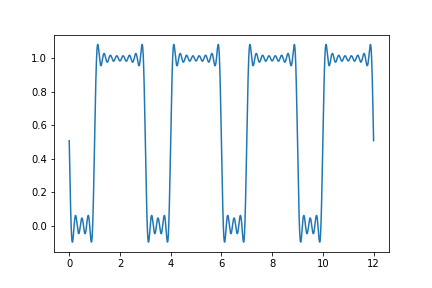
\includegraphics[scale=0.7]{Unfiltered12.png}

Low-pass:

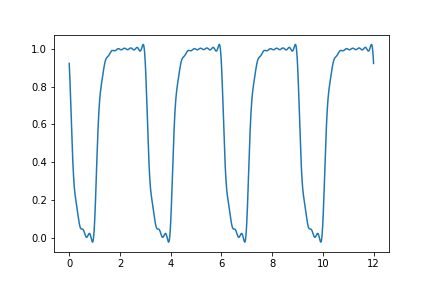
\includegraphics[scale=0.7]{LowPass12.png}

High-pass:

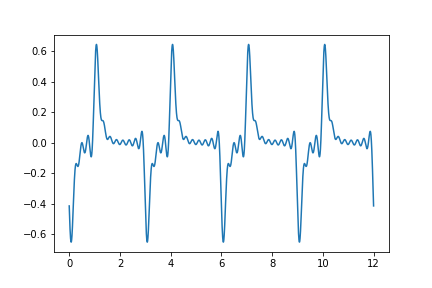
\includegraphics[scale=0.7]{HighPass12.png}


\clearpage

Taking two hundred terms of the Fourier series:

Unfiltered:

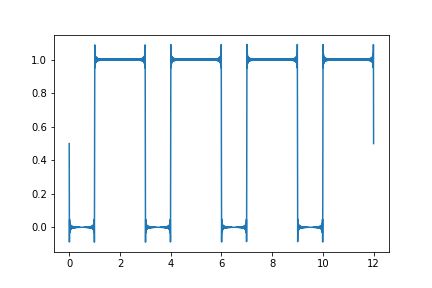
\includegraphics[scale=0.7]{Unfiltered200.png}

Low-pass:

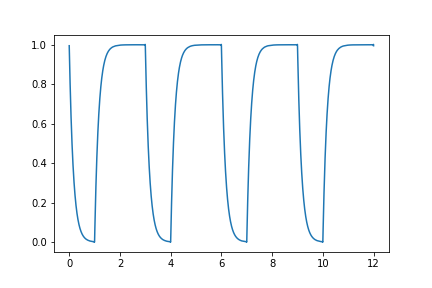
\includegraphics[scale=0.7]{LowPass200.png}

High-pass:

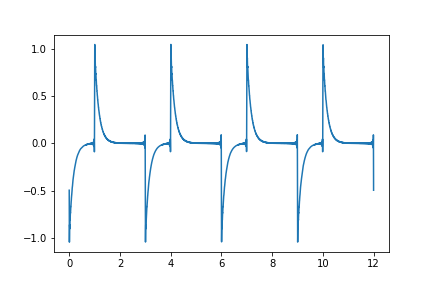
\includegraphics[scale=0.7]{HighPass200.png}












\end{document}